%# -*- coding: utf-8-unix -*-

\chapter{服务端设计与实现}
\label{chap:server}

\section{服务端概要}
\label{sec:serverOverview}

Appetizer服务端的作用主要有三个:

\begin{itemize}
	\item 接收并存储集成了Appetizer客户端SDK的Android应用程序发送的数据。
	\item 计算分析接收的数据,得到更有价值的结果。
	\item 提供数据给开发者查看。
\end{itemize}

其中提供数据给开发者查看,是服务端提供查询API,由另外的客户端调用查询API完成展现数据给开发者的功能,该部分与核心功能关系不大,本篇文章不讨论该部分。本章主要介绍Appetizer服务端如何处理接收集成了Appetizer客户端SDK的Android应用程序发来的数据,简要介绍对数据的处理方法。

\section{服务端架构}
\label{sec:serverArch}

\begin{figure}[!htp]
	\centering
	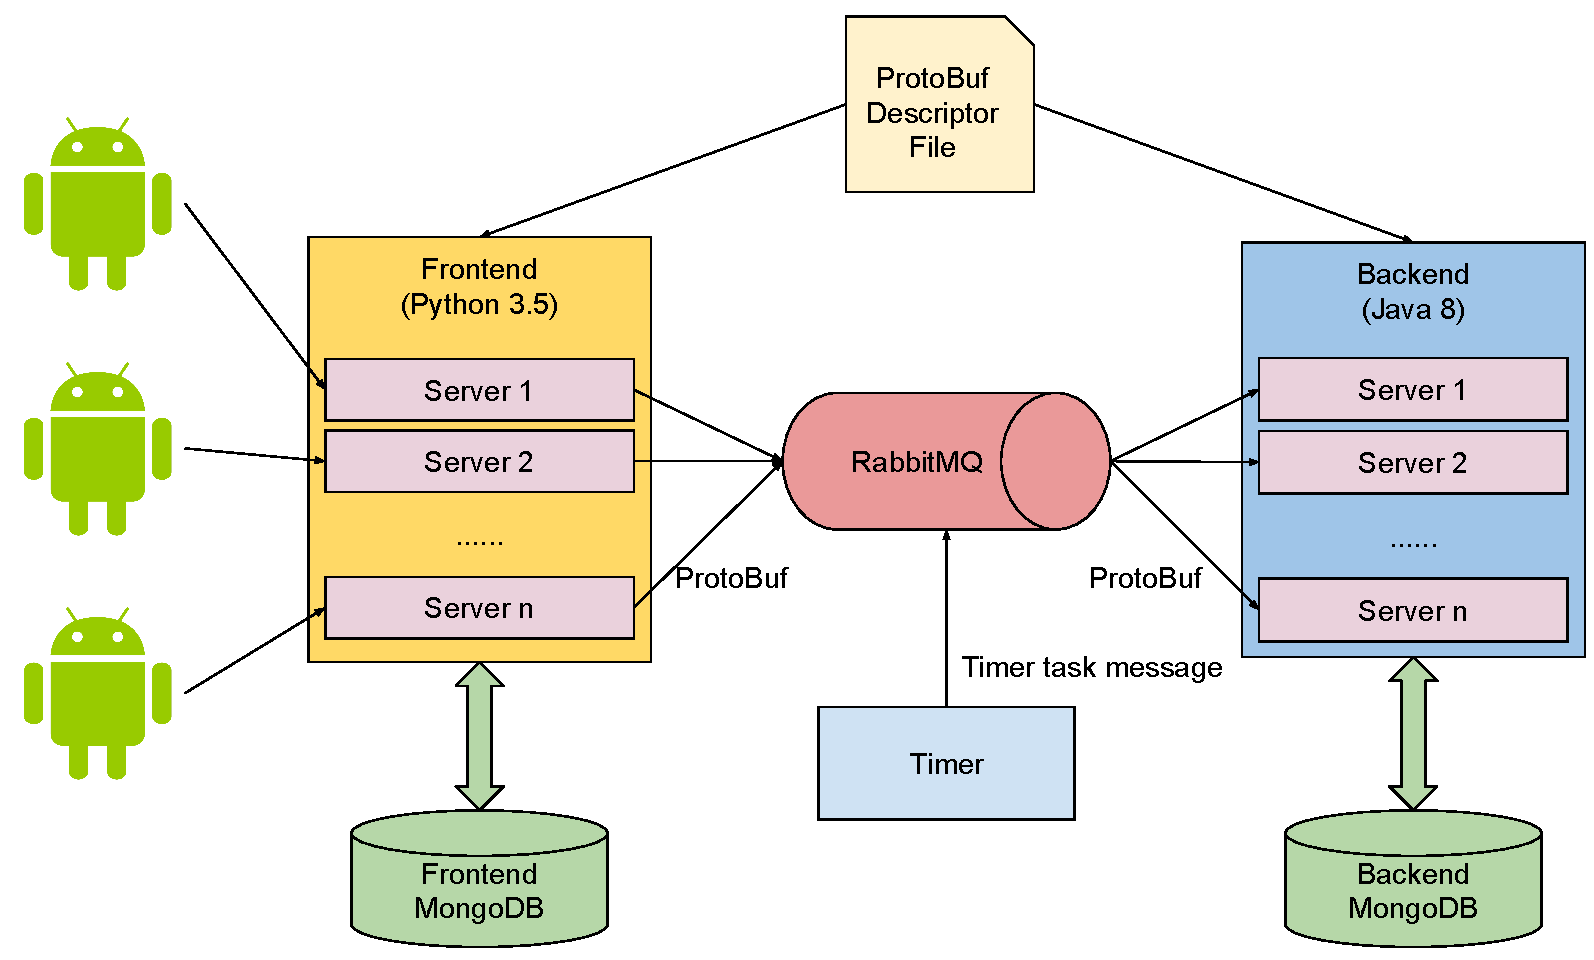
\includegraphics[width=1.0\textwidth]{AppetizerServer.pdf}
	\bicaption[fig:AppetizerServer]{这里将出现在插图索引中}{Appetizer服务端架构}{Fig}{Appetizer server architecture}
\end{figure}


如图\ref{fig:AppetizerServer}所示是服务端架构,服务端的程序主要分为前台(Frontend)和后台(Backend)两部分,其他重要的部分包括数据库(Database),前台后台的消息队列通信(MessageQueue)和定时器(Timer)。

前台、后台、数据库和消息队列四个部分采用的都是可扩展性良好的设计方案,并且结合每个部分处理的业务定制了专门的解决方案。

\subsection{前台}
\label{subsec:serverFrontend}

前台的主要作用是完成输入输出(IO)密集型业务。包括接收集成了Appetizer客户端SDK的Android应用程序发送的数据,对数据做简单的处理转发给后台,提供查询API供面向开发者的客户端使用,前台系统大部分时间在处理存储、网络任务,只有少量计算型任务。

Appetize服务端的前台(Frontend)部分使用Python 3.5开发,接收Andorid应用程序的数据部分基于asyncio HTTP实现。选择使用Python实现前台的首要原因Python是动态类型,提供原生Map类型便于操作JSON格式数据,可以有效提高前台业务的开发效率。Python的劣势是性能,但是前台的业务偏向输入输出(IO)密集型而不是计算密集型,因此性能的劣势不会称为整个系统运行效率的瓶颈,除此之外Python 3.5新增的协程异步关键字能很方便的开发异步程序,适合输入输出密集型的程序。

前台的业务逻辑主要包括数据格式处理、时间校准、数据库存储和数据转发到后台,业务逻辑的任务流主要使用 Python 3.5提供的async IO进行分配执行,数据库相关的操作使用第三方库motor实现,motor是一个结合async IO和MongoDB的工具库。

整个前台程序,包括HTTP请求路由、业务逻辑执行、数据库操作都支持Python的异步协程(async)机制,便于写出支持多核的不阻塞异步业务逻辑代码。

\subsection{后台}
\label{subsec:serverBackend}

后台的主要作用是持久化存储数据和完成计算密集型业务。后台接收前台做过简单处理的数据,持久化存储数据,对数据做增量型数据统计处理,定时做计算量较大的数据处理业务,处理后的数据定时发送给前台共查询API调用。

Appetizer服务端的后台(Backend)部分使用Java 8开发,主要考虑到Java较好的计算性能以及强大的工具类库,依赖的第三方库包括ProtocolBuffer、MongoDB Driver和RabbitMQ Client。
后台框架将RabbitMQ通道传来的消息分配到不同的任务执行单元,框架自动将消息内的ProtocolBuffer数据根据描述文件转成MongoDB的BSON(二进制JSON)对象,然后进行增量处理或者定时的全量处理。

定时任务的触发由另一块单独的Python程序完成,定时器同样通过RabbitMQ发送消息触发Appetizer服务端Java后台程序的定时任务,复用Java后台的消息分配机制,并且RabbitMQ生产者消费者模型有断电容错恢复机制,定时器复用消息模型增强了定时任务的稳定性。

\subsection{数据库}
\label{subsec:database}

前台和后台的数据库使用的都是MongoDB,因为Appetizer面向的数据都不是简单的用户信息,单个数据都涉及到较为复杂的多级结构,例如Android系统ROM构建信息本身还包含若干信息,直接使用JSON格式存储该信息的内容比较合适,Android系统ROM构建信息本身又是整个崩溃设备实时状态的一部分。因此存储单元为文档(Document)的NoSQL数据库MongoDB作为Appetizer服务端系统的数据库非常合适。

MongoDB的单个文档(Document)最多存4MB的数据,建议低于1MB,部分业务的数据可能大于1MB,例如统计日活跃用户的用户列表信息对于百万级用户量以上的Android应用数据会大于1MB,对于可能发生这种情况的任务,程序逻辑会对文档进行拆分。

\subsection{通信}
\label{subsec:rabbitmq}

前台和后台之间的通信采用RabbitMQ,支持多机与多机之间的生产者消费者模型消息传递。消息的内容使用ProtocolBuffer对象,前台和后台的数据模型可以使用同一份ProtocolBuffer描述文件,通过工具自动生成Python和Java的数据对象代码。为了避免写过多的后台Java模型类序列化和反序列化代码,后台部分实现了自动从ProtocolBuffer生成的Java模型类到MongoDB使用的BSON格式对象基础类型的转换。

采用生产者消费者消息模型的原因是让整个系统架构具有可伸缩性,即使某个时间段来自Android应用程序的消息数量过多,后台相比前台耗时更大,后台的任务不需要立刻反馈,无法处理的消息可以堆积在消息队列中,需要加大处理能力可以简单的增加机器,生产者消费者消息模型保证系统的稳定性和可伸缩性。

\section{服务端实现}
\label{sec:serverImplementation}

Appetizer的服务端实现偏向具体业务,不是本篇文章介绍的重点,相比于Appetizer客户端SDK的实现内容篇幅更少,主要介绍核心部分。其中时间校准对应Android客户端SDK所有带有时间信息的数据,用户统计对应Android客户端SDK收集的用户会话信息,崩溃信息处理对应Android客户端SDK收集的应用崩溃信息和应用程序未响应信息。

\subsection{时间校准}
\label{subsec:timecorrect}

时间校准是前台业务非常重要的预处理部分。集成了Appetizer客户端SDK的Android应用程序收集的数据中的时间信息,如果从远端服务器获取精确的时间存在两个问题,首先是开销太大,所有包含时间的信息都要做至少一个网络输入输出(IO)操作,其次是不能保证所有设备都在网络通畅的环境,因此Appetizer客户端SDK收集的数据从远端服务器获取时间是不可取的,只能从本地设备获取。

虽然真实情况下大部分Android系统ROM都会自动从服务器校准时间,时间比较准确,但Android设备的时间可以由用户自己修改,所以从本地获取的时间对于服务端依然是不可信的,服务端所有的时间信息需要校准到服务器的本地时间,服务器的本地时间是可控的,认为是准确可信的。

Appetizer时间校准的解决办法需要Android客户端SDK配合,对于所有涉及时间的信息,Appetizer客户端SDK在发送到服务端之前会添加发送时的本地时间数据到发送的数据包中,Appetizer服务端前台接收到数据时,服务端当前时间减去数据中发送时间得到差值,认为这个差值是服务端本地时间和Android设备本地时间的差值,再对数据中所有从Android设备获取的时间加上该差值,这样就把所有在Android设备本地获取的时间校准到服务端的时间。时间校准是Appetizer服务端前台为数不多计算量稍大的任务。

该时间校准方法依然存在两个问题:

\begin{enumerate}
	\item Android应用程序发送数据中的发送时间和服务端接收数据的服务端本地时间不是物理世界中的同一时刻,存在网络延迟的时间间隔,该间隔的大小是不确定的。
	\item Android设备可能在一次信息收集过程中记录多个时间节点之间,修改设备本地时间。例如记录用户会话信息时在开始和结束之间修改设备本地时间。
\end{enumerate} 

问题1虽然会影响时间校准的准确性,但是在本篇文章介绍的系统中是可以容忍的。因为需要精确计时的业务都是计算时间间隔,时间校准的精确程度对于时间间隔没有影响。其他需要记录时刻的业务都不需要高精度的计时,可以容忍数秒的时刻偏移。

问题2如果要彻底解决,需要Appetizer客户端SDK监听设备本地时间修改事件,还需要额外的权限。考虑到问题2发生的概率较小,即使发生也不会造成很严重的影响,因此整个系统容忍问题2的存在。

\subsection{用户统计}
\label{subsec:usercomputing}

用户统计是能够依靠简单的数字直观展现Android应用程序用户活跃趋势的度量维度。从宏观上考虑,用户活跃度主要受应用体验和运营策略两个因素的影响,应用体验包括界面设计、应用卡顿、应用崩溃等因素,Appetizer客户端SDK可以收集这些数据,开发和运营团队可以根据用户统计对应用界面和运营方式进行调整。

用户统计的业务实现主要包括两部分,实时用户使用量和以天为单位的日活跃用户(DAU)、日活跃新增用户(DNU)、日活跃老用户(DOU)。

实时使用量的统计难以做到精确,因为实时统计需要每台设备在使用的过程中能够顺利发送数据到Appetizer服务端,网络环境不允许的设备数据的实时性遭到了破坏,因此Appetizer服务端实现的实时使用量统计会比真正的实时使用量低。
实时使用量的业务在后台实现,前台转发时间校准后的用户会话数据到后台,实时使用量不需要考虑同一个用户多次开启应用程序合并次数,后台在存储用户会话数据的同时进行增量统计,定时器间隔五分钟触发定时任务,后台将每个Android应用程序近7天的以小时为单位的应用使用量发送到前台,前台更新接收的数据到前台数据库,供查询API调用。

日活跃相关数据业务统计更为复杂,会话数据需要和设备信息进行关联。定时器每天触发日活跃相关数据任务一次,对于每个应用程序,后台程序对当日时间内的会话数据以设备ID为键进行聚合统计,得到该应用程序日活跃用户列表。Appetizer对于“老用户”的定义为7天之内使用过应用程序的用户,因此日活跃新增用户(DNU)通过日活跃用户(DAU)列表减去之前7天的日活跃用户(DAU\_last\_7\_days)列表计算得到。日活跃新增(DNU)用户通过日活跃用户(DAU)列表减去日活跃老用户(DOU)列表计算得到。三个日活跃相关数据计算得到后只发送用户数量给前台,因为前台只关注用户数量不需要具体的用户列表。

\ref{subsec:database}小节介绍了MongoDB单个文档(Document)支持的最大空间为4MB,用户统计的用户列表作为一个List对象存储在一个文档(Document)中,List中的元素是设备ID,因此当某个Android应用的日活跃用户超过一百万时,存储一百万个设备ID在一个List会造成整个文档的大小超过4MB。用户统计业务逻辑考虑到这个问题,对于用户量较多的单个Android应用程序进行日活跃度相关的计算时,单个文档过大会进行分文档存储。

\subsection{崩溃信息处理}
\label{subsec:crashcomputing}

不同的Android设备发送的崩溃信息可能是由于同一个原因导致的,因此对崩溃信息做聚类可以更直观的展现给开发者查看,每个崩溃原因作为一个独立的事项,还包括该崩溃发生的设备系统分布、机型分布等有价值的信息,可以用来判断是否是设备或者系统的原因而不是程序本身造成的应用崩溃。

Android应用崩溃根据函数调用栈的信息进行分类,从调用栈最底层开始到最顶层看做一个单项链表,链表节点内容为文件名、函数名、行号的元组。链表节点主要分为两类,一类是开发者写的Android应用程序部分的代码,特征为包名开头为项目的名字,可以直接通过包名进行区分,另一类是Android系统本身的代码、Android支持库(support library)的代码和其他第三方库的代码,特征为包名开头是android、java或者项目目录Manifest里依赖的第三方库的包名。

两个崩溃信息根据满足以下规则2或规则3中的一个并且满足规则1,则认为是同一个崩溃原因,否则认为是不同的崩溃原因:

\begin{enumerate}
	\item 首先抛出的异常或者错误的类名相同。
	\item 链表的第一个节点如果是开发者的代码,则从第一个节点依次到首个Android系统或者支持库的代码节点之前,节点内容全部相同。
	\item 链表的第一个节点如果是Android系统或者支持库的代码,则从第一个节点依次到首个开发者的代码节点(包括首个开发者的代码节点),节点内容全部相同。
\end{enumerate}

相同的崩溃原因造成的崩溃集合,称为一个崩溃项。Appetizer服务端接收到Android设备发送的崩溃信息后,会做如下处理:

\begin{enumerate}
	\item 找到该崩溃信息对应的Android应用程序。
	\item 将崩溃信息的哈希值和该Android应用程序中已有崩溃信息的哈希值进行对比,如果存在相同的哈希值,将此次崩溃加入到该崩溃项的列表中,业务逻辑程序结束。
	\item 根据上述的链表匹配规则和该Android应用程序中的每个崩溃信息链表进行对比,如果判断为同一个崩溃原因,将此次崩溃加入到该崩溃项的列表中,业务逻辑程序结束。
	\item 创建新的崩溃项,将此次崩溃加入到新的崩溃项的列表中。
\end{enumerate} 

步骤2的哈希值相当于崩溃信息索引,通常情况下一个Android应用的大部分崩溃信息都是由少部分崩溃原因造成的,如果对于每个崩溃信息都进行链表匹配算法会造成巨大的开销,因此通过哈希索引崩溃信息可以大幅提高业务流程处理的的速度。

在崩溃信息加入到崩溃项中之后,会对该崩溃项的设备分布、版本分布统计信息做增量计算,可以给开发者提供每个崩溃项的设备分布统计和版本分布统计数据。

\section{本章小结}

本章内容主要介绍了Appetizer服务端的架构以及核心业务功能,服务端是整个系统不可或缺的一部分,用于存储、处理Appetizer客户端收集的数据,提炼出有价值的信息提供给开发者和运营团队进行查看。

\ref{sec:serverOverview}节介绍了服务端收集Android设备发送的数据、对数据进行处理、提供给开发者和运营团队查看处理后数据的三个主要功能。

\ref{sec:serverArch}节介绍了服务端整体架构,对各个组件的技术选型原因进行了分析。
\ref{subsec:serverFrontend}小节介绍了前台系统的主要功能,解释了前台业务偏向输入输出(IO)密集型的特点,分析了选择Python实现前台系统的原因以及前台在实现上选择工具库做出的权衡。
\ref{subsec:serverBackend}小节介绍了后台系统的主要功能,后台业务偏向计算密集型的特点,说明了后台系统选择Java开发的原因,消息队列RabbitMQ在后台系统的作用和定时器的设计。
\ref{subsec:database}小节介绍了MongoDB的优势以及Appetizer服务端选择MongoDB作为前台和后台数据库的原因,还说明了可能需要拆分文档的应用场景。
\ref{subsec:rabbitmq}小节介绍了Appetizer服务端前台和后台之间的通信机制,通信传递的内容采用ProtocolBuffer同时具备性能和便于开发的优势,以及相关通信架构提供的系统可伸缩性和可扩展性。

\ref{sec:serverImplementation}节介绍了Appetizer服务端有展现价值的部分。
\ref{subsec:timecorrect}小节介绍了在Appetizer整个业务流程中发生的时间偏差的原因,Appetizer客户端SDK只从本地设备获取不可信时间,设计并实现了依靠客户端SDK和服务端合作的时间校准方法,分析了该方法可能发生的问题,得到该时间校准方法有效可行的结论。
\ref{subsec:usercomputing}小节介绍了Appetizer核心功能用户统计的价值、作用和实现方法。
\ref{subsec:crashcomputing}小节介绍了Appetizer另一个核心功能崩溃信息处理的设计实现,描述了一种对Android应用崩溃信息的原因进行分类的方法。
